\documentclass[11pt]{article}
\usepackage{graphicx}
\usepackage{hyperref}
\usepackage[dvipsnames, svgnames, x11names, hyperref]{xcolor}
\hypersetup{
	colorlinks,
	citecolor=Violet,
	linkcolor=Red,
	urlcolor=Blue}
\usepackage{natbib}
\usepackage{commath, amsmath}
\usepackage{siunitx}
\usepackage{gensymb}

\setlength{\textwidth}{6.5in}
\setlength{\headheight}{0in}
\setlength{\textheight}{8.0in}
\setlength{\hoffset}{0in}
\setlength{\voffset}{0in}
\setlength{\oddsidemargin}{0in}
\setlength{\evensidemargin}{0in}

\title{PS-4 Solution}

\author{Nana Ama Darpaah}

\begin{document}
	\maketitle
	This is my GitHub link: \href{https://github.com/nnd2016/phys-ga2000.git}{Nana Ama's GitHub Link}
	
\section{Question 1}
Th heat capacity of a solid at temperature T, as expressed by Debye's theory, is given by

\begin{equation}
	C_{v} = 9V\rho k_{B}(T/\theta_{D}^{3})\int_{0}^{\theta_{D}/T}(x^{4}\exp(x))/(exp(x)-1)^{2} dx
\end{equation}
where V is the volume, $\rho$ is the number density of atoms, $k_{B}$ is Boltzmann's constant and $\theta_{D}$ is the Debye temperature.

At V = $1000 cm^{3}$,  $\rho$ = $6.022e28 m^{-3}$ and $\theta_{D} = 428 K$ at N = 50 sample points, the function cv(T) was created using Gaussian quadrature which yielded the heat capacity at a specific temperature.

A plot of heat capacity against temperature ranging from T = 5 K and T = 500 K was made using the function above. The result is as shown in Figure \ref{fig:heat_capacity}.
\begin{figure}[h]\begin{center} 
		\vspace{12pt}
		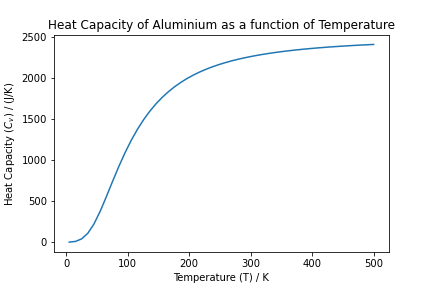
\includegraphics[width=0.67\textwidth]{heat_capacity.png} 
		\caption{A graph of the heat capacity of aluminium against temperature }
		\label{fig:heat_capacity}
	\end{center}
\end{figure} 
	
\section{Question 2}
Using 
\begin{equation}
	T = \sqrt{8m}\int_{0}^{a} dx/\sqrt{V(a) - V(x)}
\end{equation}
Gaussian quadrature was used to evaluate the integral within the function using N = 20 points and a graph of the period against amplitude was plotted from a = 0 to a = 2. 
The graph is shown below.
\begin{figure}[!h]\begin{center} 
		\vspace{12pt}
		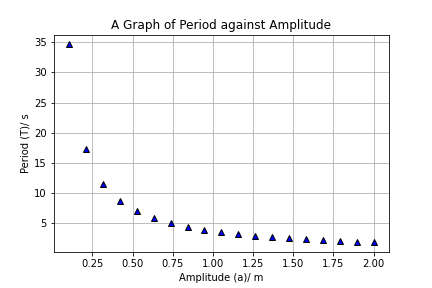
\includegraphics[width=0.7\textwidth]{anharmonic period.png}
		\caption{A graph of period against amplitude of an harmonic oscillator }
		\label{fig:anharmonic_period} 
	\end{center}
\end{figure} 

It can be seen from the graph in Figure \ref{fig:anharmonic_period}  that as amplitudes increase, the oscillator gets faster.

\section{Question 3}

For n = 0, 1, 2, 3 at x = -4 to x = 4, the graph of $\psi_{n}$ against x yields the result in Figure \ref{fig:oscillator_multiple_n}
\begin{figure}[!h]\begin{center} 
		\vspace{12pt}
		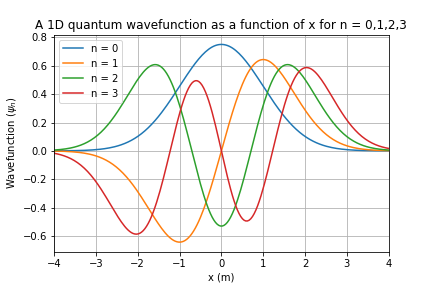
\includegraphics[width=0.7\textwidth]{oscillator_wavefuntion_multiple_n.png} 
		\caption{A graph of first 4 wavefunction plots of n against x}
		\label{fig:oscillator_multiple_n}
	\end{center}
\end{figure}

For n = 30 at x = -10 to x = 10, the graph of $\psi_{n}$ against x yields
\begin{figure}[!h]\begin{center} 
		\vspace{12pt}
		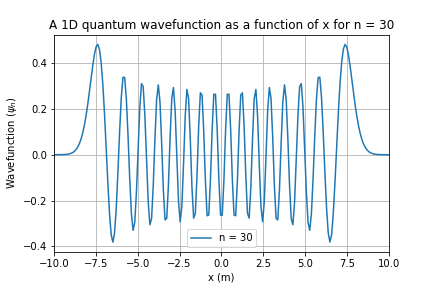
\includegraphics[width=0.7\textwidth]{oscillator_wavefunction_n_30.png} 
		\caption{A plot of the wavefunction at n = 30 against x }
		\label{fig:oscillator_n30} 
	\end{center}
\end{figure}
 The uncertainty was found to be 2.3452078737858177
	
\end{document}